\documentclass[12pt, a4page]{article}


\usepackage{amssymb}
\usepackage[backend=biber]{biblatex}
\addbibresource{biblio.bib}

\title{Metcalfe's Law}
\date{}
\author{Pranav Kasela, Federico Moiraghi}

\usepackage{graphicx}
\begin{document}
\maketitle
\begin{abstract}
%later we will add and modify the abstract.
Sarnoff was an American businessman and a pioneer of the radio and television, he is credited with the Sarnoff’s law, which states that the value of a broadcast system grows linearly with the number of users.
Robert Metcalfe born in 1946 is an electrical engineer, applied mathematician, computer scientist and businessman, he is the co-founder of Ethernet together with David Boggs.\newline
Sarnoff’s law was the base of the Metcalfe’s law which states that in the case of Ethernet the growth is quadratic with the linear growth of users. The law was formulated by George Glider in 1993 after a discussion with Metcalfe. This law which is mathematically correct but has some strong hypothesis for business applications. \newline
Reed’s law states that the utility of large network grows exponentially with the size of network $2^n$, which is more than the number of users ($n$) and the possible pair of connection ($n^2$).
Both these law’s have been criticized by a MIT mathematician, Andrew Odlyzko who states that both Reed and Metcalfe overstates the growth of internet since the don’t take in account the human tendency to saturate the number of connections they make with others using the Dunbar’s number. He empirically states due to different analogies that the growth should be $n\cdot \log n$ for n very large and states that Metcalfe’s law is valid only for small network (small $n$). We will explain Odlyzko’s hypothesis and generalize Metcalfe’s law using the mathematical series concept.\newline
We will prove the law stated above and their economical implications and explain in which case they have a real evidence.
\newpage
\end{abstract}

\part*{Math Proofs}
% we will modify the title
% we will add images later too
We start with the Sarnoff's rule, which is pretty simple.
It states that the value of a broadcast network is linearly proportional to it's users, so basically if we have $n$ users we will have that the value growth is $V \cdot n$ (where $V$ is the value of a connection).
A simple example would be a radio or companies like Netflix.
\newline
\begin{figure}[htp]
\centering
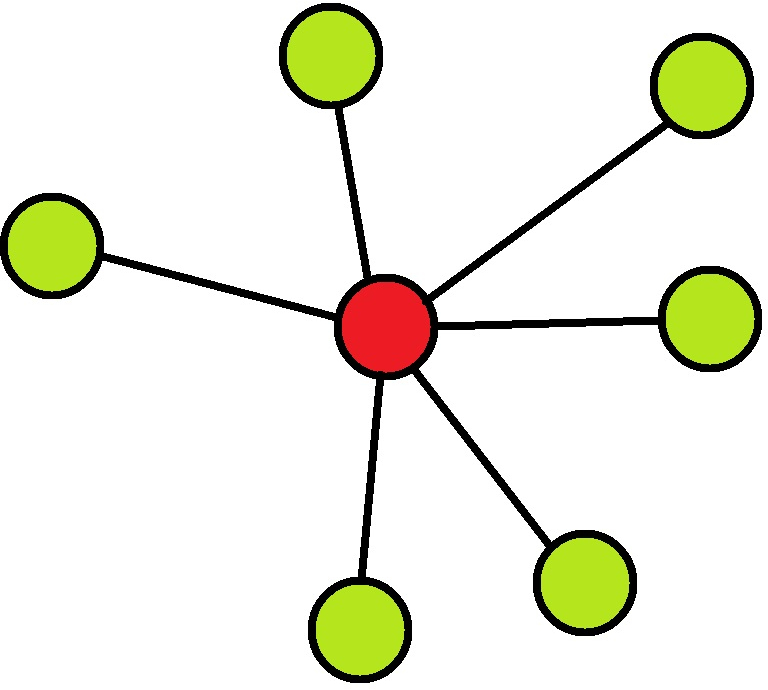
\includegraphics[scale=1.00]{IMAGE1.jpg}
\caption{Red is the broadcaster, green are the users.}
\label{IMAGE1}
\end{figure}
\newline
%perchè qui sotto non usiamo \paragraph{Proof} ? 
%Si poteva anche usare quello :'D, ma in matematica alcuni preferiscono scrivere il teorema in grassetto e proof in corsivo solo per quello.
\textit{Proof} : The proof is trivial since we have $n$ users connected to single node, which is considered to be the streamer.
Assume every connection has value $V$ then we will just sum $V$ $n$-times obtaining a value of $\sum_{i=1}^{n} V = V \cdot n$ \hfill $\square$
\newline
\newline

Next is Metcalfe's Law, which states that the growth rate is proportional to the square of number of users.\newline
\textit{Proof} : The idea is similar to the Sarnoff's law: fixing one of the $n$ nodes, we can see that using Sarnoff's law (or common sense) we have $n-1$ connections.
\begin{figure}[htp]
\centering
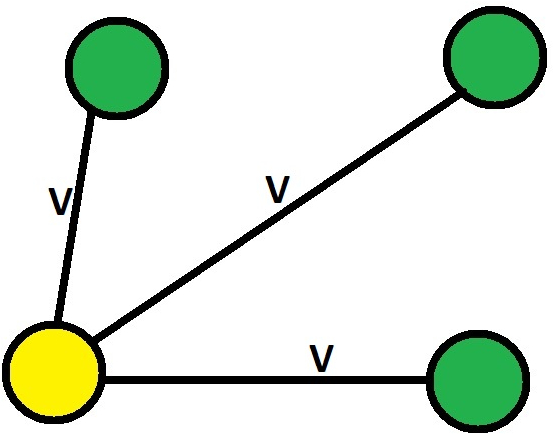
\includegraphics[scale=1.00]{IMAGE2.jpg}
\caption{we are connecting the yellow node to the greens.}
\label{IMAGE2}
\end{figure} \newline
Assuming that every connection has the same value $V$, we have that from the first node we are gaining $V \cdot (n - 1)$ value; now, fixing a second node, we obtain again $n-1$ connections; but remember that we have already considered the connection with the first node, so we have $n-2$ connections, thus we generate $V \cdot (n - 2)$ value. \newline
\begin{figure}[htp]
\centering
%ridotto la scala altrimenti la figura andava giu e non volevo forzarla con !
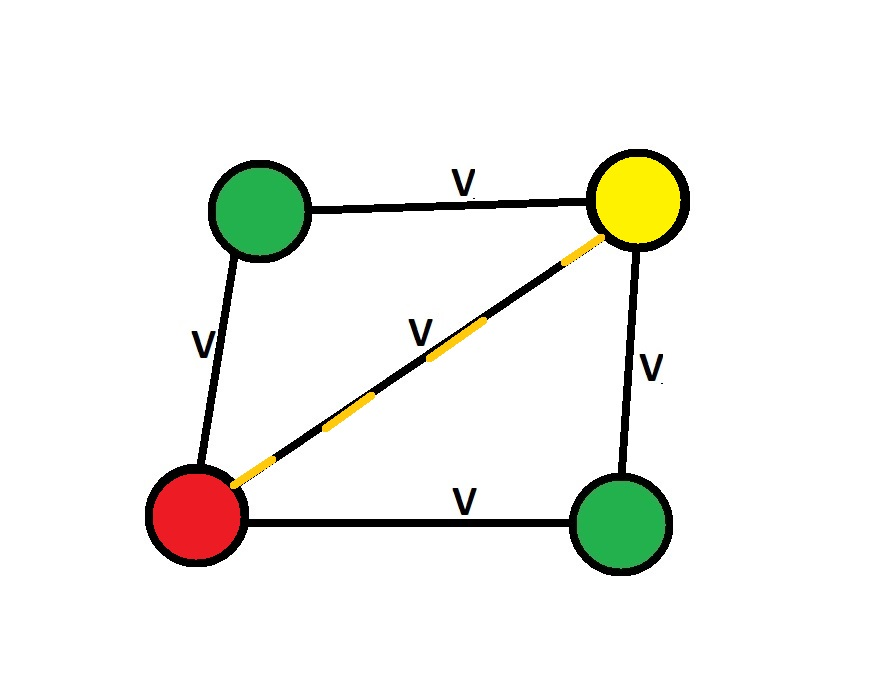
\includegraphics[scale=0.95]{IMAGE3.jpg}
\caption{we can see that connecting the yellow we are doubling the dashed yellow connection to the red node, so we need to remove it in our calculations.}
\label{IMAGE3}
\end{figure} \newline
So, proceeding this way and summing all the values, we have that the total value is $\sum_{i=1}^{n-1} V \cdot i = V \cdot \sum_{i=1}^{n-1} i = V \frac{n(n-1)}{2} \propto \frac{V}{2} n^2$  \hfill $\square$
\newline \begin{figure}[htp]
\centering
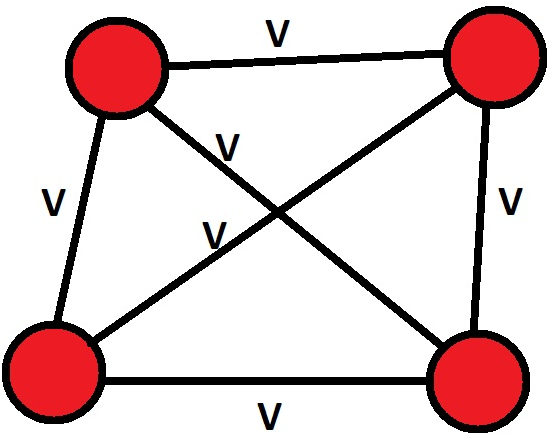
\includegraphics[scale=1.00]{IMAGE4.jpg}
\caption{A totally connected network with n=4}
\label{IMAGE4}
\end{figure} \newline

Now we try to prove a general formula, without assuming that every connection has the same value and assuming that $n$ is large enough; otherwise the optimal solution is Metcalfe's Law, which has a strong hypothesis and cannot be satisfied if the number of users is very high simply because we cannot connect one of them to all others.
For example if we had only 10 users on a social media then most probably all of them will connect between themselves without discrimination; but if we were to have millions of users, without using some algorithm to extrapolate value out of them, we cannot have that these millions (it would be $\propto$ million$^2$ using Metcalfe's law) of connection will have the same value: it's not only a time restriction but a space restriction too. Since the human behavior on a large scale is similar, just see the Big Data mindset, we might use the following generalization:
fix a user, sort the others on the value of connection and call the values $V_1$ for the first connection, $V_2$ for second, ... , $V_{n-1}$ for the last one.
\newline
% da qui alla fine della parte non mi sembra spiegato molto chiaramente: rivedere un attimo
%prova adesso e dimmi se non capisci lo stesso
Since we assumed this to be true for every user, we have that the total value of network is $\propto n \cdot \sum_{i=1}^{n-1} V_n$. We can see if we have $V_{n-1}=...=V_2=V_1$ the Metcalfe hypothesis we have the $ \sum_{i=1}^{n-1} V_n = n\cdot V$ thus the network value is $\propto V \cdot n^2$ which was the Metcalfe's Law.
The network value is based on the series $\sum V_i$ if number of users $n$ is big enough, so if the series converges we will have that the value connection is linear, if it diverges we will need to study the asymptotic behavior of the series.
Surprisingly, Sarnoff's law is not only valid for broadcast networks but can be true also for fully connected network.\newline
One hypothesis that we can make is the Odlyzko's one, that the values of connection drops harmonically, in our case assume $V_1 = V$, due to this assumption we will have $V_2 = V/2, V_3 = V/3$ and so on, so the series will be $\sum_{i=1}^n V/i$, we know that for n large enough we have that $\sum_i^n 1/i \sim \log n$, so we have that the series is $\sim V \log n$, thus the value is $\propto n \log n$ (see \cite{Odlyzko_Law}).\newline
We showed 3 different values of the value for the connection so which one is the right one? There is a big difference between $n, n\log n, n^2$ we can say that this three represent a pessimistic, average and optimistic growth of a network.
%no need for reed's law will put only in the presentation

\newpage
\part*{Socio-Economic Interpretation.}
Metcalfe's Law assumes that each node is linked with the whole net and all connections have the same importance.
Those assumptions are considered too strong, so new mathematical laws have been presented; but empirical studies have demonstrated the veracity of Metcalfe's Law in popular social networks\cite{Metcalfe}\cite{Wechat} even if premises of are not satisfied.
However, in a social environment the human nature of nodes must be considered; moreover, algorithms used to improve connections quality and the possibility given by the platform to \textit{share} contents may be enough to make the value of the whole network increase according to a quadratic function $n^2$. \newline

Estimating the value of a net is important in an economic contest: costs and earnings are the base of any business. Costs are not considered just in terms of money, but also as resources needed to run the business, like server's disk space and computational power.
Decisions concerning the server depends on the costs of the whole network; and since it is necessary to run the business, estimation can not be lower than real costs: the service risks to be interrupted and the value of the network drastically decreases to zero. \newline

\section{A real case: Facebook.}
Facebook, the biggest network in the world owned by a public company, is demonstrated to have a value proportional to the square of active users\cite{Metcalfe}\cite{Wechat}.
But assumptions of Metcalfe's Law are apparently not satisfied due to the limit to the number of \textit{friends} that a single person can have and the fact that users do select their contacts according to various strategies\cite{Socialmedia}. \newline

However, this is not a problem, because Facebook's algorithm and the possibility to \textit{share} contents make links between people that apparently are not connected: the exchange of value is imposed by Facebook, even without user's consent.
According to Pasquali\cite{Socialmedia}, Facebook is not a single network, but an aggregate of small (social) networks that exist also offline and a big (informatic) net composed by the aggregate of all users.
While small social networks are not interesting in this study, the fact that users can interact with the whole Facebook is fundamental.
Users, in fact, can \textit{share} contents, so that they can reach more nodes (\textit{friends of friends} or \textit{public pages}), or, in particular cases, a \textit{post} can become \textit{viral}.
In addiction to this, Facebook's algorithm minds the creation of new links, suggesting new contents that is sure to be liked by the user or suggesting new people or pages.

The value exchanged through Facebook's network is maximized by the algorithm: not all information are presented to the user, but they are filtered according to personal interests.
The unique experience during the \textit{flow} of feeds can cause dependency: the time spent on the platform, the facility of access and the quality (or targeting) of contents are so high that saturation is not easily reach. \newline

\section{Economic Evaluation of a Net.}
In general, networks are not the product of the business but just the distribution channel: in this case, the net can be evaluated equal to earnings coming from it; in this case the model is just linear.
This is just a simple and empirical way to estimate a value, but works even for big companies that offer a payment service. \newline
A generalization of this criterion is to calculate the sum of value exchanged between each node; this can be easily done in e-commerce sites or for a transport nets\cite{Weinman}
. \newline

Metcalfe's Law is necessary when no or small data are available, so the value can not be known and can be just estimate.
This is the case of advertisement selling: the value of the space is not known, but companies have to define a price according to the distribution that the advert may have in the network. \newline

Estimating the value is important when balance-sheet is compiled or budget is calculated. In addiction, according to Italian's Law, the balance-sheet must be \textit{prudent}, so costs can not be under-estimated.
With this in mind, Metcalfe's Law is correctly adopted: if costs follow a $o(n^2)$ model, law would not be broken; in fact, it is empirically demonstrated\cite{Wechat} that costs of a social media follows this law.
Using the same criterion, if no data are available, earnings are not well estimated: is more prudent using a lower formula, like $n \cdot \log{n}$. \newline

\section{Net saturation.}
In a network, nodes are often normal people: in a finished time not all the value transmitted can be extracted.
This means that a person has no time to communicate with and may not receives all communications from the whole network.
The term \textit{saturation} is used to mean that a person can not exchange the maximum value with all other nodes due to the mole of information that receives.
In addition, not all communications have the same value: user is covered with information, for the most useless, that can not manage. \newline
To maximize the value that a network can transfer, filters of any type are used: from simple spam filters, to automatize the check of emails, to server algorithms that suggest new actions and connections.
In this way, the value of links increases due to the growth of information that the user can manage. \newline

\section{Conclusions.}
The value of a network is not easily estimable: in general, the value is inferior to $n^2$ presented by Metcalfe, but with some tricks is possible to a net to reach the maximum value.
In particular, Facebook's network, due to its possibility to \textit{share} contents and a sophisticated algorithm that uses tons of information about each user, can be evaluated according to Metcalfe's Law; but this mathematical function is not always valid, even in social environment, due to human nature: social networks are not so inter-connected, and a informatic infrastructure mirrors the offline world. 
And more in general, other laws, of minor magnitude, are empirically and successfully used.
\newpage
\printbibliography

\end{document}
